\documentclass{beamer}

\usepackage{graphicx}
\usepackage{courier}

\title{New features for SHOP}
\subtitle{Luis Morales, Dorothy Dunford}

\begin{document}
	\frame {
		\titlepage
	}
\begin{frame}[allowframebreaks]{Overview}
The model has two big components:
\begin{itemize}
\item Analysis cycle:

\begin{itemize}
\item Launch every 6h (12:00am, 6:00am, 12:00pm, 6:00pm)
\item Run in steady-state mode. Estimate average hydraulic variables in the last 24h.
\item Initial conditions: The model is initialed with the average hydrauclic variables estimated 24h ago.
\item Boundary conditions: Used observed hydraulic variables averagesd in the last 24h. Source of data: hydrometric data (CanHyS); water levels (SJR); wind data (HRDPS)
\item Domain: St. Lawrence river from Montreal to Trois-Rivieres.
\end{itemize}

\framebreak
\item Forescast cycle:

\begin{itemize}
\item Launch every 6h
\item 54h forecast (6h analysis + 48h forecast) 
\item I.C. and B.C. for the 6h analysis, see below (the analysis cycle is embeded in the forecast cycle for a different domain!)
\item Initial conditions for the 48h forecast: The model is initialed with the output of the previous 6h analysusis cycle.
\item Boundary conditions for the 48h forecast: from: Water Cycle Prediction System, SPINE, and HRDPS (wind fields)
\item Domain: St. Lawrence river from Carillon and Beauharnois to Saint-Joseph-de-la-Rive.
\end{itemize}
\end{itemize}
\end{frame}

%-----------
\begin{frame}[allowframebreaks]{Maestro's model structure}
\begin{figure}
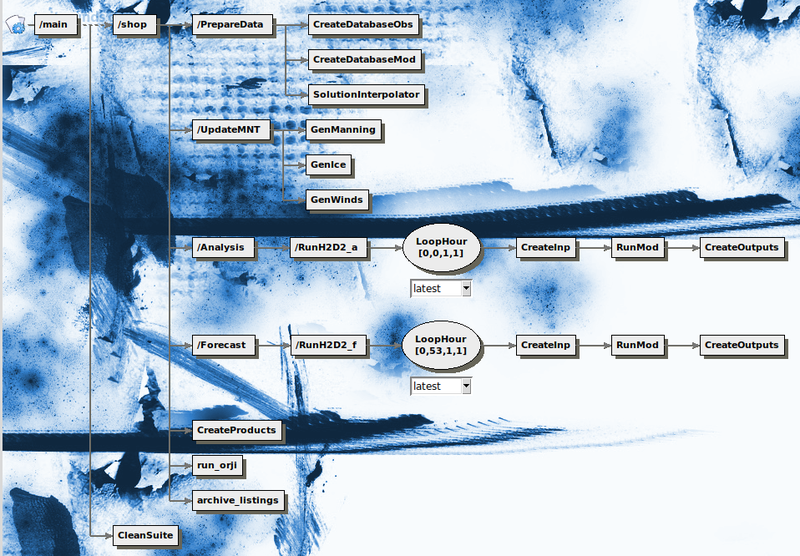
\includegraphics[scale=0.5]{800px-Flow.png}
\end{figure}

\framebreak

Main Maestro's modules under \texttt{/shop} (root module)
\begin{itemize}
\item \texttt{/PrepareData}:
\begin{itemize}
\item \texttt{CreateDatabaseObs}
\item \texttt{CreateDatabaseMod} 
\item \texttt{SolutionInterpolator} 
\end{itemize}
\item \texttt{/UpdateMNT}: 
\begin{itemize}
\item \texttt{GenManning} 
\item \texttt{Genice}
\item \texttt{GenWinds} 
\end{itemize}

\item \texttt{/Analysis} 
\item \texttt{/Forecast} 
\end{itemize}
both \texttt{/Analysis} and \texttt{/Forecast} include this module \texttt{/RunH2D2} and these tasks:\texttt{LoopHour[]} \texttt{CreateInp} \texttt{RunMod} \texttt{CreateOutputs}

Other tasks include: \texttt{CreateProducts} \texttt{CleanSuite}
\end{frame}
%-----------


%-----------

%-----------

\end{document}
